\chapter{Implementierung aufbauend auf bestehenden Technologien, REST API und Dynamic Hosting}

\section{Sinatra und PostgreSQL zur Optimiertung des bestehenden Technologiestacks}
Wie bereits in vorangegangenen Kapiteln beschrieben, bieten Microservices die Möglichkeit zum optimierten Einsatz von Technologien. Für die zu entwickelnde Anwendung gab es diverse Optimierungsmöglichkeiten. Hier sollte zum Einen insbesondere auf die Wahl der Datenbanktechnologie, zum Anderen vor Allem auf die Wahl des Frameworks geachtet werden.

\subsection{Wahl des Webframeworks}
Die Hauptanwendung ist im Ruby Framework Ruby on Rails\cite{rails} entwickelt worden. Ruby on Rails ist jedoch als Framework zu \textit{heavy-weight} und mit zu viel Overhead verbunden, als das es sich für einen schnellen, minimalistischen Microservice eignen würde. Ruby on Rails ist an erster Stelle für monolithische Anwendungen entwickelt.~\cite[][]{rails:doctrine}
Hierbei ist nicht nur die Performance entscheidend, sondern auch die Struktur des Codes. Rails als traditionelles Model-View-Controller Framework\cite[][]{wiki:mvc} eignet sich somit vor Allem auch nicht aufgrund seiner Struktur. Die minimalistischere Rails API Variante\cite{rails:api} hat zwar einen geringeren Overhead als Rails, für einen geschwindigkeitsorientierten Microservice bieten sich weitere Optimierungen jedoch an.

\begin{figure}[!ht]
    \centering
    \caption{Geschwindigkeitsvergleich Rails, Rails API und Sinatra \cite{newrelic:soa}}
    \label{fig:speed}
    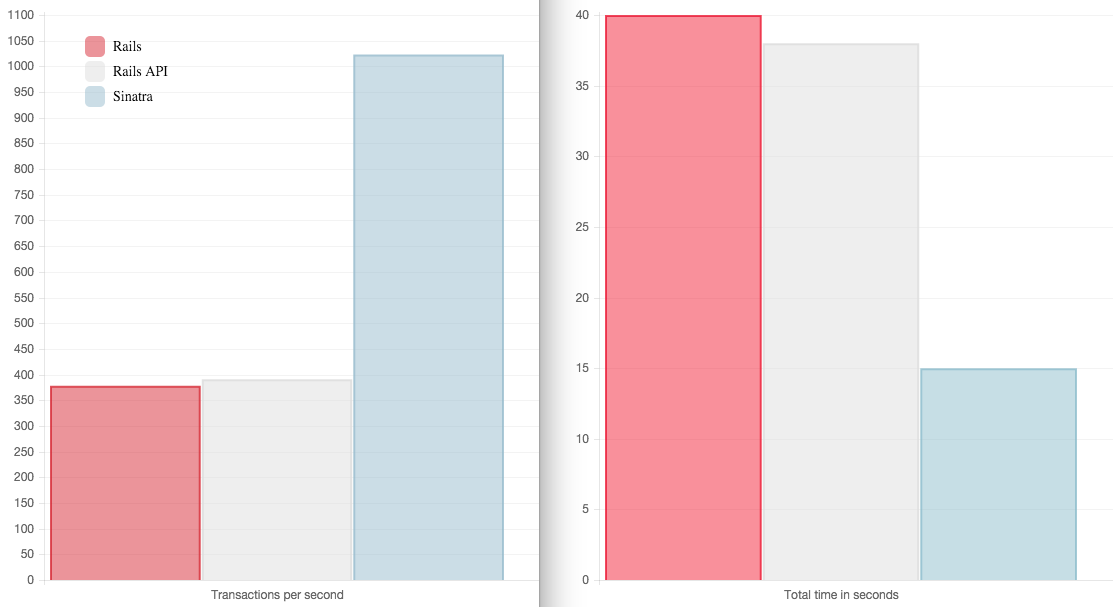
\includegraphics[width=\textwidth]{rails_sinatra}
\end{figure}

Alternativen bilden sogenannte Microframeworks\cite{wiki:micro}. Microframeworks zeichnen sich im Gegensatz zu full-stack Frameworks dadurch aus, das viele der Funktionen nicht Teil des mitgelieferten Umfangs sind. In den meisten Sprachen gibt es diverse Microframeworks, wie z.B. Flask\cite{flask} für Python, Express\cite{expressjs} für Node, Sparkjava\cite{sparkjava}, oder das Sinatra Framework\cite{sinatra} für Ruby. Die Sprache Go\cite{golang} kommt bereits mit gut ausgebauten net/http Paketen und umfasst dadurch die meisten üblichen Funktionen schon ohne Framework.

Zwar gibt es Geschwindigkeitsunterschiede in diesen Frameworks\cite[vgl.][]{frameworks}, im Vergleich zu klassischen full-stack Frameworks sind diese aber unerheblich. Da die Datenbank in der bestehenden Anwendung den größten Flaschenhals bildet (vgl. \autoref{fig:newrelic}), muss hier nicht zwangsläufig das beste Framework gewählt werden. Stattdessen sollte auf die bestehende Firmenstruktur geachtet werden. Da fast die gesamte Backendtechnologie bisher mit der Programmiersprache Ruby entwickelt ist und es somit keine anderen im Produktionsbetrieb eingesetzt wird, wäre die Integration einer neuen Programmiersprache in das Unternehmn mit nicht unwesentlichen Kosten verbunden. Vor Allem, da der neue Microservice auch mit einem komplett eigenen Produktionssetup verbunden ist, stellt eine in der Firma bisher unbekannte Programmiersprache eine ganz eigene Herausforderung dar. Um die Wartbarkeit des Systems hoch zu halten und die Risiken für den Betrieb zu minimieren, entschied ich mich daher auch im neuen Microservice die Programmiersprache Ruby einzusetzen. Da das Framework Ruby on Rails überproportioniert ist und nicht den Anforderungen entspricht, entschied ich mich für den Einsatz des Ruby Frameworks Sinatra.
\begin{figure}[!ht]
    \centering
    \caption{Queries bilden Flaschenhals im Sampling}
    \label{fig:newrelic}
    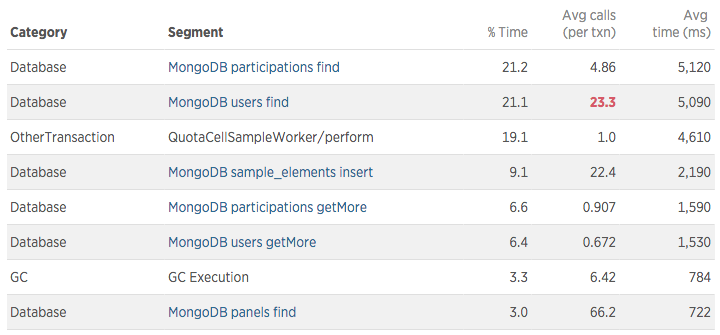
\includegraphics[width=\textwidth]{newrelic_sampling}
\end{figure}
Sinatra ist nach Ruby on Rails das mit Abstand beliebteste Ruby Framework\cite[vgl.][]{ruby2015} und wird daher von den meisten Ruby Web Tools unterstützt.

Wie bereits erwähnt, ist Sinatra ein sogenanntes Microframework. Sinatra selbst lässt also viel Raum für Konfiguration, unterstützt jedoch in den wesentlichen Zügen der Webentwicklung. Sinatra erleichtert so zum Beispiel das Routing enorm. Hier kann schnell eine Routing Struktur erschaffen werden, die Definition von Routen und deren Antworten ist sehr komfortabel und schnell einzurichten. Sinatra ist vor Allem auch nicht darauf ausgelegt in Antworten HTML zu rendern, so kann leicht eine JSON Response definiert werden.
Eine Route zum Anlegen von Resourcen kann z.B. so definiert werden:
\begin{lstlisting}[language=Ruby]
class SomeController < Sinatra::Base
  post '/resources' do
    data = JSON.load(request.body.read)
    [...] # some actions to save the resource
    # return appropriate 201 code
    [201, { data: `success' }.to_json }]
  end
end
\end{lstlisting}

Weiterhin erleichtert Sinatra das Betreiben eines Webservers und bietet eine Schnittstelle zum Ruby Standard Webserver Interface Rack\cite{rack}. Hier wird dem Entwickler viel Arbeit abgenommen. Viele Tools zum Betreiben von Webservices, z.B. im Bereich des Monitorings oder des Loggings unterstützen ebenfalls das Sinatra Framework. So bringt Sinatra also nicht viel Overhead \textit{out of the box}, bringt aber die Möglichkeit zur Nutzung vieler praktischer Erweiterungen.

Als Webserver wählte ich den Ruby Webserver Puma\cite{puma}. Puma ist ein Webserver mit verhältnismäßig geringem Speicherverbrauch, dadurch bietet er sich vor Allem für den Betrieb eines Microservices an.
\subsection{Datenbanktechnologie}
Da die Datenbank das scheinbar größte Problem der Performance in der bestehenden Anwendung bildet, ist es hier dringend notwendig die eingesetzte Technologie zu überdenken. 
Zwar ist MongoDB von der Idee her keine schlechte Wahl für die Userprofile, die Art wie Profildaten abgefragt werden, passt aber nicht gut zum dokumentorientierten Ansatz von MongoDB.

Die Schemalosigkeit von MongoDB in Zusammenarbeit mit den recht variablen Profilen war ursprünglich der Hauptgrund diese Technologie einzusetzen. Nutzerprofile sind stark unterschiedlich, viele mit ja beantworteten Fragen führen zu weiteren Fragen (z.B. ``Haben Sie Kinder?'', ``Wie viele Kinder haben Sie?'', ``Wie alt ist Kind x?''). Hierbei bietet es sich durchaus an MongoDB mit seiner \textit{Embedded Document Struktur} zu benutzten, statt unzählige 1 zu n Beziehungen zu verwalten.
Bei der Abfrage der Daten verspricht MongoDB Geschwindigkeitsvorteile, wenn man einzelne Dokumente aus der Datenbank erhalten möchte. So kann zum Beispiel die Struktur einer Powerpoint Präsentation wie folgt abgebildet werden:
\begin{lstlisting}[language=Ruby]
{
    presentationId: 1,
    title: "A Presentation",
    author: "me",
    slides: [
        {
            slideId: 1,
            slideOrder: 1,
            elements: [
                {
                    elementId: 1,
                    elementXPos: 100,
                    ...
                },
                ...
                }
            ]
        },
        ...
    ]
}
\end{lstlisting}
Eine Präsentation kann nun mit nur einer Abfrage, ohne jegliche Joins aus der Datenbank geladen werden. Die ganze Präsentation kann vorgerendered werden und die Anwendung zur Erstellung oder Präsentation von Präsentationen ohne weiteres Nachladen genutzt werden. Hier liegt MongoDB's Stärke: Strukturen können in ihrer natürlichen Form abgebildet werden und dokumentorientiert schnell aus der Datenbank geladen werden.
So ist auch der Aufbau der Profile konzipiert worden. Für die Verwaltung der Daten und für die Pflege der Profile durch die Nutzer ist dieser Aufbau durchaus angebracht.
Beim Erstellen einer Query und dessen Ausführung über die Gesamtpopulation ist dieser Aufbau jedoch nicht optimal. Hier sind nie alle Profilfelder eines Nutzers relevant, sondern lediglich ein Querschnitt über alle Nutzer. Queries sehen in der Regel wie folgt aus:
\begin{lstlisting}[language=Ruby]
{
    "profile.participations.response_rate.value": {
        "$lt": 0.3
    },
    "profile.basic.locale.value": {
        "$in": ["de", "de-AT"]
    },
    "profile.basic.age.value": {
        "$gt": 21,
        "$lte": 100
    }
}
\end{lstlisting}

Hier wird auf eine verhältnismäßig geringe Zahl von Profilfelder, meist weniger als 10, über die gesamte Population gequeried. Weiterhin werden dann nicht gesamte Nutzerobjekte zurückgegeben, sondern lediglich die Anzahl der passenden Nutzer, deren Ids oder Antwortraten. Die MongoDB Query Struktur ist dafür schlichtweg nicht optimiert.

Hinzu kommt, dass MongoDB Datenbanken auf 64 Indizes beschränkt sind\cite{mongo:indexlimit}. Da Nutzerprofile in Nutzern eingebettet sind, gehen für die Verwaltung der Nutzer zum Login schon diverese Indizes verloren. Bei der verhältnismäßig hohen Komplexität der Profile, mit 176 Feldern, reicht dieses Limit nicht aus.
Weiterhin sind Ansätze wie ``Index Intersection'' und ``Partielle Indizes'' in MongoDB relativ neue Konzepte und noch nicht voll ausgereift\cite{mongo:indexintersection}\cite{mongo:partialindexes}.
Zwar gibt es besondere Häufungen der Queries bei bestimmten Feldern und diese sind auch durch Indexe abgedeckt, vor Allem aber die Queries auf die anderen Felder verlangsamen die Anwendung erheblich.

Hier besteht schlicht eine Diskrepanz zwischen den Queryanforderungen. Zum Einen wird hier dokumentenorientiert, zum Anderen spaltenorientiert gearbeitet.
Die Pflege der Nutzerprofile durch die Nutzer geschieht dokumentorientiert. Für die Nutzer ist immer genau ein Nutzerprofil relevant, nämlich ihr eigenes. Das Nutzerprofil wird in seiner Gesamtheit aus der Datenbank angefragt, verändert und wieder abgespeichert.
Das Nutzersampling hingegen geschieht spaltenorientiert. Über die Gesamtheit aller Nutzer wird eine bestimmte Menge von Spalten abgefragt und anschließend eine Spalte (z.B. die ids oder die Antwortraten der Nutzer) aus der Datenbank geladen.
% (FIX TOO ABSOLUTE, it's not column oriented after all)
Ein Ansatz diese Diskrepanz zwischen Nutzersampling und Profilpflege zu lösen, bietet die Command Query Responsibility Segregation (CQRS).~\cite[][]{fowler:cqrs} Gemäß der Anforderungen verschiedener Services bietet es sich hier an, die Darstellung von Daten, die theoretisch identisch sind, auf verschiedene Anwendungfälle zu optimieren. Auf Code Ebene können zum Beispiel separate Models genutzt werden um die Daten in individuelle Repräsentationsformen zu bringen. Auf Ebene der Datenbank kann ein komplett anderes Schema zur Repräsentation der Daten genutzt werden.

\begin{figure}[!ht]
    \centering
    \caption{Aufspaltung zur Lösung der Anforderungsdiskrepanz}
    \label{fig:orientationsplit}
    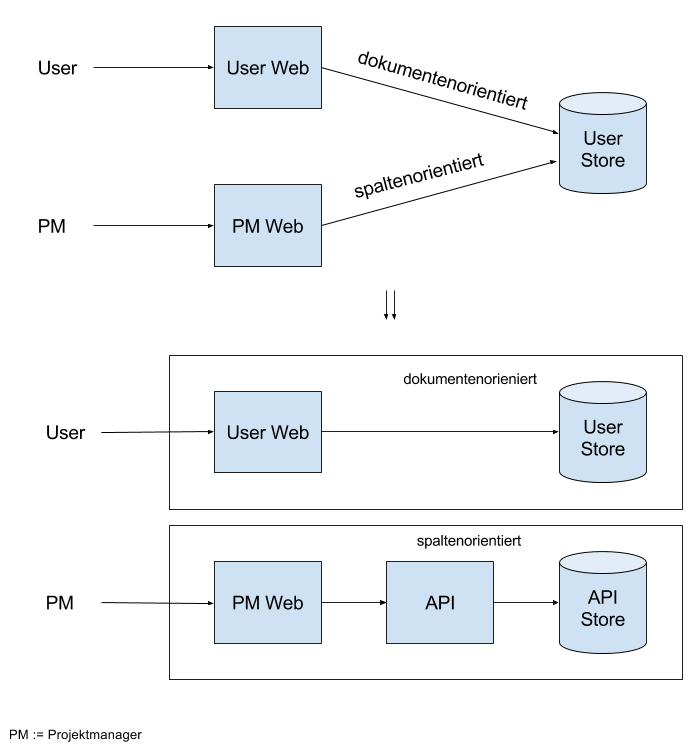
\includegraphics[width=\textwidth]{orientation_comparison}
\end{figure}

Weiterhin führen Änderungen der Nutzerprofile in MongoDB auch immer zu einem \textit{write-lock}. Auch wenn dieser noch so kurz sein mag, er behindert doch immer das gleichzeitige Auslesen der Daten. Auch das spricht für eine neue, separate Datenbank zum Lesen der Daten für Samplingzwecke.

Aufgrund der offensichtlichen Mängel im Schema im Bezug auf die Nutzerqueries bot es sich an, die Datenbanktechnologie zu wechseln und stattdessen eine SQL Datenbank zu verwenden. Im Gegensatz zum Wechsel der Programmiersprache, stellt der Einsatz einer anderen Datenbanktechnologie im konkreten Fall keine große Hürde dar. Im Betrieb besteht bereits eine MySQL\cite{mysql} Datenbank als Data Warehouse und eine PostgreSQL\cite{postgres} Datenbank für eine für einen Kunden betriebene Anwendung. Daher besteht Erfahrung sowohl in der Entwicklung mit, als auch dem Betrieb von SQL Datenbanken.
Ich entschied mich für den Einsatz einer PostgreSQL Datenbank. PostgreSQL bietet hier die Möglichkeit eine spaltenorientierte \textit{Engine} zu nutzen\cite{postgres:column}. So kann zwar im Betrieb auf bekannte SQL Technologien gesetzt werden, Optimierungsmöglichkeiten in Richtung Spaltenorientiertheit sind dennoch möglich.

Die Hauptaufgabe besteht nun darin, die bestehende, verschachtelte Struktur der MongoDB Datenbank in ein SQL Format zu übersetzen.
In \autoref{fig:fields} sind die bisher eingesetzten Ruby Klassen zur Abbildung der MongoDB Datenstruktur abgebildet. 

\begin{figure}[!ht]
    \centering
    \caption{Vereinfachtes Klassendiagramm zur Darstellung der vorhandenen Profilfelder}
    \label{fig:fields}
    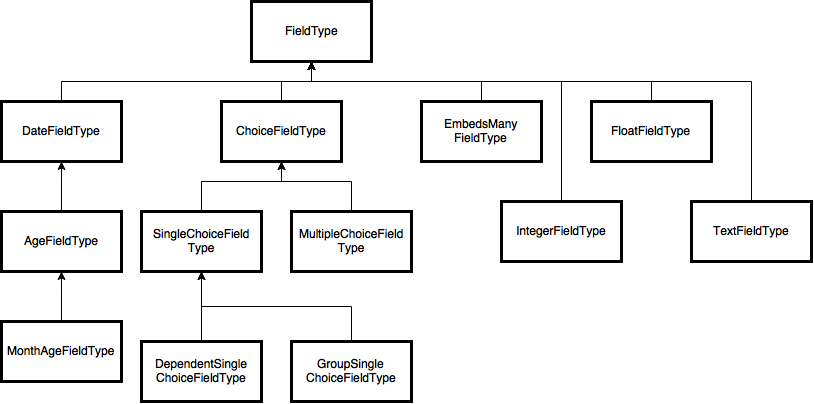
\includegraphics[width=\textwidth]{field_types}
\end{figure}

Eine Herausforderung bilden hier vor Allem die Felder der Klasse ChoiceFieldType. Die anderen Felder können problemlos in eine flache Struktur überführt werden. Für Choice Felder, sollte nun gemäß der Normalisierung von Datenbanken (FIX WELCHE NORMALFORM? QUELLE) eine eigene Tabelle mit Relation angelegt werden. Die MultipleChoice Felder müssten weiterhin mit einer `has-many' Relation abgebildet werden, was zu vielen Joins bei Queries führen würde. Da Joins im Allgemeinen verhältnismäßig langsam sind (FIX QUELLE), ist dies in Anbetracht der Aufgabenstellung ein Problem. Da die Datenbank im Microservice jedoch lediglich zu möglichst schnellen Abfrage der Daten, nicht aber zur Pflege und Organisation der Daten genutzt wird, ist es hier vertretbar eine denormalisierte Struktur zu wählen. So entschloss ich mich für den Einsatz von Bitstrings. Jede Auswahlmöglichkeit wird hier durch ein Bit repräsentiert. So kann zum Beipsiel die Mehrfachauswahl von Städten in Berlin, mit den drei Auswahlmöglichkeiten Hamburg, Berlin und München, auf einen drei Bit langen Bitstring abgebildet werden. Der Bitstring `010' in der Datebank bedeutet dann, dass nur die Option Berlin, nicht aber die Optionen Hamburg und München ausgewählt wurden. Dies spart zum Einen Platz in der Datenbank, zum Anderen reduziert es den Einsatz von Datenbankjoins. Es muss natürlich ein Overhead beim Übersetzen der alten Queries in ein Bitstring Format eingeplant werden. Weiterhin wird hier eine Kopplung zwischen Code und Datenbank eingeführt. Wenn sich die Optionen in der Datenbank ändern, muss immer zusätzlich zu allen anderen Stellen diese eine Stelle im Code aktualisiert werden.

Eine weitere Schwierigkeit stellen hier die EmbedsMany Felder dar. Auch hier ist eine `has-many` Relation notwendig, diese kann aber nicht, wie bei sich wiederholenden Auswahlfeldern, durch einen Bitstring ersetzt werden. (FIX MORE STUFF)

%(FIX NOBODY CARES? TOO MUCH GELABER??)

Zusätzlich zur relationalen Datenbank setzte ich in der Entwicklung weiterhin Redis\cite{redis} als Zwischenspeicher ein. Redis ist ein in-memory data store, der sowohl zu Datenbankzwecken, als auch zu caching Zwecken genutzt werden kann. Da die Daten ausschließlich im Arbeitsspeicher des Systems abgelegt werden, können hier sehr hohe Geschwindigkeiten erreicht werden.
Zunächst überträgt die Hauptanwendung in Form eines POST requests die Query. Diese wird dann in Redis gespeichert. Die errechneten Queryergebnisse werden dann ebenfalls in Redis gespeichert. Die Ergebnisse können dann jederzeit von der Hauptanwendung abgefragt werden. Außerdem ist es möglich und perspektivisch geplant, die Geschwindigkeit von Redis für das Caching zu nutzen. Es kann überprüft werden ob übertragene Queries bereits bekannt sind und anhand dessen Alters die Ergebnisse übernommen werden. Weiterhin kann hier Performance gewonnen werden, da keine langfristige Persistenz gefordert ist. So kann Redis einzig und allein im Arbeitsspeicher speichern und muss nicht, wie sonst üblich, jede Änderung auf der Festplatte speichern.\cite{redis:faq}

%(FIX FIRST I SAY ONLY IN-MEMORY, THEN I SAY ALSO ON DISK)

\subsection{Architektur des Microservices}
Wie bereits beschrieben, handelt es sich beim entwickelten Microservice hauptsächlich um eine Query Schnittstelle. Der Overhead soll hier möglichst gering gehalten werden um die Geschwindigkeit zu optimieren.

Da die bereits existierende Datenbank, aus den bereits beschriebenen Gründen weiter in der Betriebsawendung erhalten bleibt, bietet es sich an, zur Abfrage der neuen Datenbankfelder, die alten Feldnamen an den Microservice zu übergeben.
Die bestehende Schnittstelle zu MongoDB bietet hier eine praktische \textit{.to\_json} Methode. Mit dieser kann eine Query leicht in ein gut übertragbares Format überführt werden. Eine erstellte Abfrage auf alle Nutzer, die als Sprache deutsch angegeben haben:

\begin{lstlisting}[language=Ruby]
User.where(:'profile.basic.locale.value' => 'de')
\end{lstlisting}

\noindent kann so leicht in ein JSON-Format überführt werden:

\begin{lstlisting}[language=Ruby]
User.where(:'profile.basic.locale.value' => 'de').selector.to_json
=> { "profile.basic.locale.value": "de" }
\end{lstlisting}

\noindent So bildet das Übersetzen der übergebenen Feldnamen einen wesentlichen Teil des entwickelten Microservices.
Diese Kopplung zwischen den Services ist zwar grundsätlich nicht ideal, aber im konkreten Anwendungsfall durchaus sinnvoll. Schließlich werden beide Datenbanken weiterhin parallel verwendet und die Umstellung soll mit einem möglichst geringen Aufwand durchgeführt werden.
Es bietet sich jedoch an, in der Zukunft einen zentralen Punkt zur Pflege der Übersetzungen der Feldnamen einzurichten, um die Aktualität der Übersetzungen zu garantieren. Eine nur im Microservice verwaltete Übersetzung kann bei neu hinzugefügten Feldern in der MongoDB Datenbank leicht vergessen werden und schnell \textit{outdated} sein.

Einen weiteren wesentlichen Bestandteil bildet das Handhaben des übergebenen JSON Strings. Dieser wird im ersten Schritt anhand einer JSON Schema\cite{jsonschema} Definition validiert. So wird sichergestellt das er wohlformattiert ist und den gestellten Anforderungen entspricht. Hier kann vor dem Schritt des wirklichen Parsens ggf. noch einmal Last reduziert werden. War die Validierung erfolgreich wird der übergebene JSON String geparsed. Hierzu habe ich einen Parser entwickelt, der das übergebene MongoDB JSON Format in eine PostgreSQL kompatible Notation überführt. Schnell wird jedoch deutlich, dass es jedoch auch relati komplexe Querykonstrukte gibt. Da wäre zum Einen der Einsatz von Vergleichsoperatoren. Hier können leicht auch solche Queries entstehen:

\begin{lstlisting}[language=Ruby]
User.where(
    :'profile.basic.locale.value'.nin => ['de', 'de-AT', 'de-CH'],
    :'profile.automotive.car_amount.value'.gt => 3,
    :'profile.automotive.car_amount.value'.lte => 10
).selector.to_json
=> 
{
    "profile.basic.locale.value": {
        "$nin": ["de","de-AT","de-CH"]
    },
    "profile.automotive.car_amount.value": {
        "$gt": 3,
        "$lte": 10
    }
}
\end{lstlisting}

\noindent Dies muss der Parser also auch übersetzen können. Im gleichen Schritt werden, neben dem Parsen, auch die Datenbankfeldnamen übersetzt.

\section{Schaffung einer standardisierten REST Schnittstelle}
Einen entscheidenden Unterschied zwischen Microservice Architektur und monolithischer Entwicklung, bildet die Schnittstelle zwischen den Anwendungsteilen. Während im Monolithen simple Code Calls stattfinden, muss für die Kommunikation zwischen verschiedenen Servies zunächst ein geeignetes Protokoll zum Austausch gefunden werden.
Da hier eben kein durch die Programmiersprache vorgeschriebener Standard besteht, ist es wichtig ein geeignetes Austauschformat zu definieren.
Um Änderungen sowohl im Client, also auch im Service möglich zu machen, sollten keine sprachgebundenen Technologien eingesetzt werden. Somit kann sichergestellt werden, das möglichst geringe Änderungen anfallen, sollte ein neuer Client oder Änderungen am bestehenden System zum Einsatz einer neuen Programmiersprache führen.

Eine populäre Schnittstellentechnologie ist der Einsatz von Remote Procedure Calls (RPC)\cite{rpc}. RPC verfolgt das Hauptziel, Remote Calls wie lokale Aufrufe wirken zu lassen. Dies ermöglicht es schnell Server-Client Anwendungen zu entwickeln. Zwar sind RPC Lösungen häufig technologiegebunden\cite[vgl.][Seite 46]{newman2015building}, es gibt jedoch auch diverse Lösungen die verschiedene Technologien unterstützen. Ein großer Nachteil von RPC wird jedoch bei komplexeren Anwendungen auffällig: Remote Calls sind keine Lokalaufrufe.\cite[][Seite 47]{newman2015building} Zwar erlaubt RPC es durch ``verstecken'' der Implementierungsdetails, schnell einfache Client-Server Anwendungen zu entwickeln, mit der Zeit wird aber deutlich, dass mitunter feinere Entwicklungsmöglichkeiten notwendig sind. Hier fehlt es dann oft an besserer technologischer Kontrolle.

Eine Alternative zu RPC, die vor Allem in den letzten Jahren an Popularität gewonnen hat, ist der Representational State Transfer (REST). Im Gegensatz zu RPC, das ursprünglich für Verteilte Systeme innerhalb eines Netzwerkes oder Netzwerkverbundes entwickelt wurde\cite{rpc:history}, ist REST eng an das Internet gekoppelt\cite[vgl.][Seite 49]{newman2015building}. Nicht zuletzt deswegen wird REST, trotz relativer Protokollunabhängigkeit, meist mit dem Hypertext Transfer Protocol (HTTP) verwendet\cite[vgl.][Seite 50]{newman2015building}. Die prominenten HTTP Verben POST, GET, PUT und DELETE lassen sich direkt zu den CRUD Operationen Create, Read, Update und Delete übersetzten. Eine REST Grundlage stellt die methodische Unabhängigkeit von Ressourcen dar. Methoden sollten sich auf allen Ressourcen gleich verhalten. So kann mit Hilfe der HTTP Verben durch verschiedene Request auf eine Ressource, unterschiedliche Handlungen abgebildet werden. Statt die Methoden $createResourceX$, $readResourceX$, $updateResourceX$ und $deleteResourceX$ zu unterscheiden, kann eine einfache und abstrakte Form der Art $VERB\ RESSOURCE$ genutzt werden um alle Methoden abzubilden. So können Methoden auf Queries also durch simple HTTP Request wie $POST\ /queries$ und $GET\ /queries$ eindeutig abgebildet werden. Ein weiterer Vorteil der relativen Nähe zu HTTP, ist gute Unterstützung dieser Technolgie. Viele Technoligien die mit HTTP zum Einsatz kommen, wie z.B. Caching und Load Balancing können leicht auch mit REST eingesetzt werden\cite{rest:loadbalancing}.

Weiterhin ist REST in der Wahl des eingesetzten Austauschformats frei\cite[][Seite 53]{newman2015building}. Populäre Möglichkeiten sind hier z.B. JSON oder XML. Da die bisherige Datenbankschnittstelle einen direkten Export zu JSON bietet, bietet es sich an diese hier einzusetzen. Generell ist der Support von JSON in Ruby sehr gut. Außerdem bietet auch die eingesetzte Datenbankschnittstelle\cite{sequel} für PostgreSQL gute JSON Unterstützung.

Da das eingesetzte JSON Format frei wählbar ist und REST ebenfalls wenig Ansprüche an die Form der Daten stellt, bietet es sich hier an, unterstützend eine Technologie zur Definition des JSON Formats einzusetzen. Hier gibt es zum Beipsiel JSON Schema. JSON Schema erlaubt es die erwartete Struktur der übertragenen Daten, z.B. bei POST Requests, abstrakt festzulegen. Dies erlaubt zum Einen leichte Nachvollziehbarkeit der Schnittstelle, zum Anderen eine automatische Validierung der übergebenen Daten. So muss nicht mit dem Parsen der Daten begonnen werden, ohne das vorher sichergestellt ist, das diese semantisch korrekt sind.

Weiterhin ist es wichtig, die erstellte API gut zu dokumentieren. Hier gibt es ebenfalls gute Tools die eingesetzt werden können. Ich nutze hierzu die RESTful API Modelling Language (RAML)\cite{raml}. RAML erlaubt es eine Schnittstelle in einem Maschinen-lesbaren Format zu dokumentieren. Dies erlaubt es automatisiert API Tests generieren zu lassen. So kann sichergestellt werden, dass die API Dokumentation immer auf dem aktuellsten Stand ist. Denn wenn die API, nicht aber die Dokumentation aktualisiert wird, würden hier die generierten Tests fehlschlagen. Dies ist für verteilte Systeme besonders wichtig. RAML arbeitet hierzu mit JSON Schema um Beispielrequests zu definieren. Weiterhin lässt sich mit Tools wie RAML to HTML\cite{raml2html} leicht eine interaktive, menschenlesbare Dokumentation der API erstellen. Hier finden sich dann automatisch auch die Beispielrequests und -responses der API in JSON Format. Die Dokumentation der entwickelten API ist so für Entwickler in Form einer Webseite\cite{prophetdoku} nachvollziehbar. 
Weiterhin kann über Tools\cite{ramlconsoletool} eine interaktive Testkonsole generiert werden, die es erlaubt die API anhand der bereitgestellten Beispiele zu Testen.

REST, vor Allem im gemeinsamen Einsatz mit JSON-Schema und RAML, bildet eine reife Technologie, die sich für den Einsatz in der API Programmierung hervorragend eignet.

%(FIX RAM console)

\section{Integration des Microservices in den Monolithen}
Wie bereits im vorangegangenen Kapitel beschrieben, beschloss ich den neuen Microservice mit Hilfe eines dem Strangler Pattern ähnlichen Prinzips in die bestehende Anwendung einzubinden.
Der Einsatz des Flipper Gems erlaubt es hierbei den bestehenden Code mit alter Datenbank, sowie den neuen Microservice mit neuer Datenbank parallel zu betreiben. Anhand der abstrahierten Schnittstelle des QueryExecuters, wird entschieden, ob ein Query auf der alten Datenbank oder dem neuen Service stattfindet. Das entsprechende Klassendiagramm ist in \autoref{fig:class} dargestellt.
\begin{figure}[!ht]
    \centering
    \caption{Klassendiagramm zur Verteilung zwischen bestehendem und neu geschaffenem Code}
    \label{fig:class}
    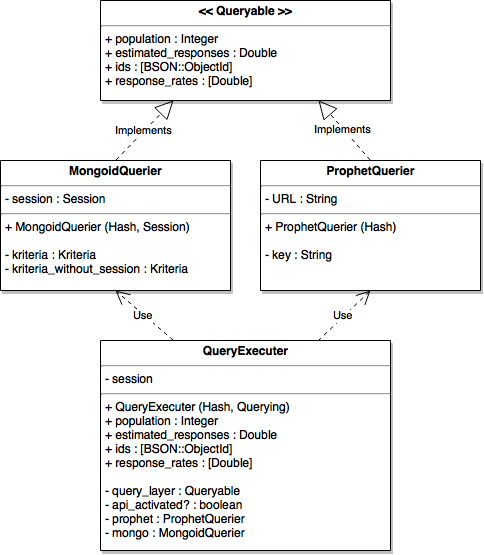
\includegraphics[scale=0.6]{klassendiagramm}
\end{figure}

Ist der Toggle aktiviert, wird zunächst per POST ein Query an den Service übertragen. Im Hintergrund initiiert der Service dann das Parsen, Übersetzen und Abarbeiten der Query. Dies geschieht asynchron. Zunächst wird die Query in Redis gespeichert und der generierte Zugriffsschlüssel zurückgegeben.
Anhand dieses Schlüssels kann die Hauptanwendung dann die freigegebenen Ergebnisse des Querys, wie die ids der zutreffenden Nutzer, abfragen. Der Ablauf kann wie in \autoref{fig:sequenz} visualisiert werden.

\begin{figure}[!ht]
    \centering
    \caption{Sequenzdiagramm zum Profilqueryen bei aktiviertem Flipper}
    \label{fig:sequenz}
    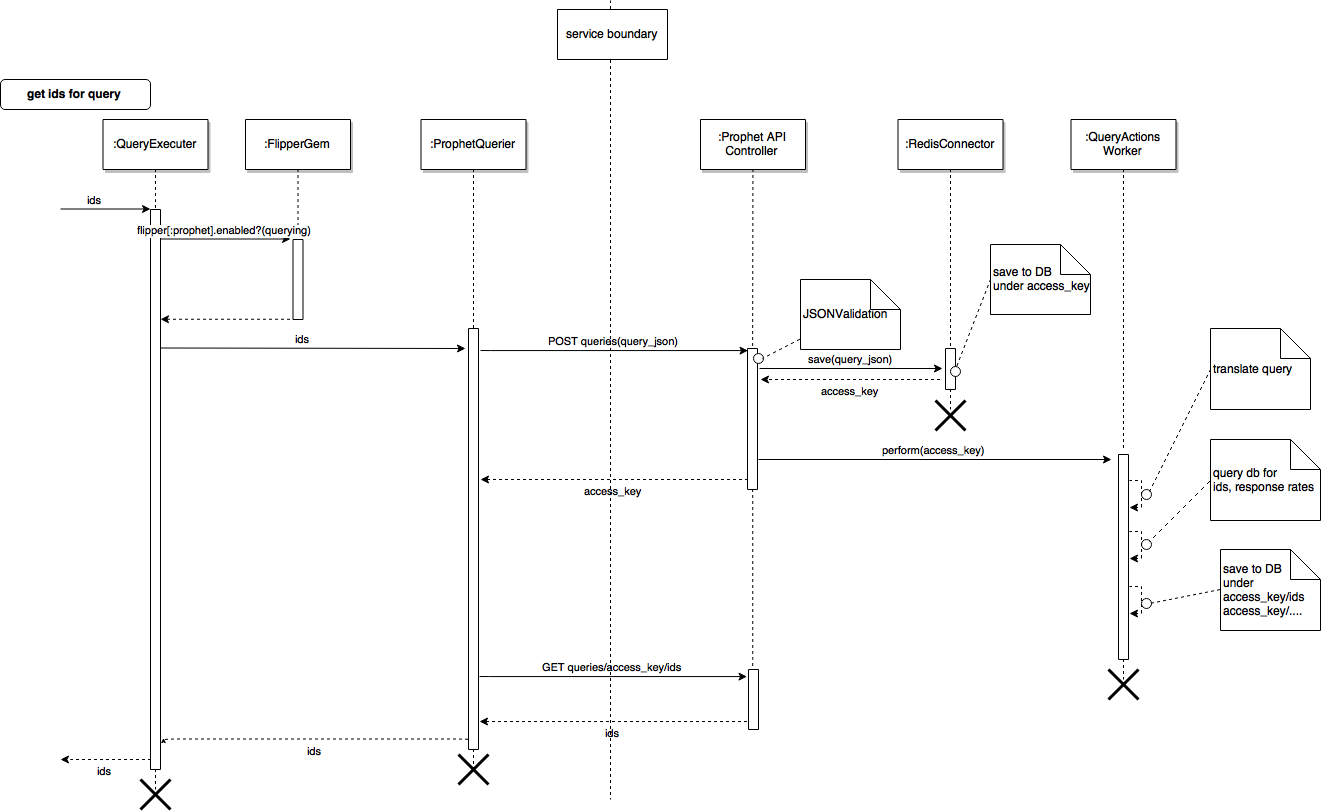
\includegraphics[width=\textwidth]{prophet_sequenz}
\end{figure}

Hier ist insbesondere das Fehlerhandling zu beachten. Es gibt hier diverse Fehlerquellen die den Ablauf beeinträchtigen können. Zum Einen kann die Query fehlerhaft sein. 
Tritt bei der JSON-Schema Validierung ein Fehler auf, wird hier ein HTTP 422 Statuscode zurückgegeben. Per Definition der Internet Engineering Task Force (IETF)\cite{ietf:424} handelt es sich hierbei um eine ``Unprocessable Entity''. Die übertragenen Daten können also nicht verarbeitet werden.
Da das Parsen der Query asynchron geschieht und die Query vorher nur Anhand von JSON-Schema validiert wird, kann eine fehlerhafte Query, beispielsweise durch illegale Datenbankfeldnamen, erst nach Antwort mit Zugriffsschlüssel erkannt werden. Geschieht dies, muss beim Abfragen der Daten von der API ein eindeutiger Fehlercode zurückgegeben werden. Es muss unterschieden werden können zwischen invaliden Schlüsseln, Timeouts und illegalen Queries. Für Abfragen nach Übermittlung illegaler Queries habe ich den Fehlercode 424 gewählt. Per Definition der IETF\cite{ietf:424}, handelt es sich hierbei um eine `failed dependency'. Der Request ist also fehlgeschlagen, da ein vorheriger Request fehlgeschlagen ist. Dies ist meiner Meinung nach der am besten passende Fehlercode.
Weiterhin kann es natürlich vorkommen, dass die Daten abgefragt werden, obwohl die Query noch nicht abgeschlossen ist. Die Daten liegen schlichtweg nicht vor. Hier wird ein HTTP 428 Statuscode genutzt. Per IETF\cite{ietf:428} steht dieser Statuscode für ``Precondition Required''. Eine benötigte Kondition wurde demnach nicht erfüllt. Dieser Statuscode passt zwar nicht so eindeutig wie der 424 Statuscode, ist aber dennoch eine angemessene Antwort.
Für den Fall, dass der Zugriffsschlüssel selbst nicht valide ist, wird ein simpler 404 Fehlercode zurück gegeben.

Für den den Fehlercode 428 (Query noch nicht abgeschlossen) und sämtliche Netzwerkfehler aus dem Fehlerbereich 500 bis 511, muss sichergestellt werden, dass erneute Abfrageversuche stattfinden.
Ein populärer Ansatz für solche Situationen, ist der des ``Exponential Backoff''\cite{expbackoff}. Bereits im Ethernet Protokoll wird Exponential Backoff eingesetzt\cite{etherbackoff}. Beim Prinzip des Exponential Backoff wird die Zeit zwischen erneuten Versuchen multiplikativ immer weiter erhöht. Die Basisgröße der zeitlichen Abstände kann hier frei gewählt werden. Der zweite Versuch findet hier in der Regel fast direkt nach Fehlschlagen des ersten statt, anschließend werden die Abstände immer größer. Hier wird die Last auf den beteiligten Systemen relativ gering gehalten, eine Operation aber nicht abschließend fehlschlagen gelassen. Grundsätzlich bietet es sich jedoch an, eine Grenze für die Zahl der Fehlerversuche festzulegen (Truncated Exponential Backoff). Wenn der Abstand z.B. auf einen Tag steigt, ist ein erneuter Versuch sicherlich nur noch bedingt sinnvoll.
Alle Queries in der Hauptanwendung werden asynchron mit Hilfe von Sidekiq\cite{sidekiq} ausgeführt. Sidekiq selbst implementiert für die ausgeführten Jobs bereits das Exponential Backoff Prinzip. Sidekiq's Retries sind jedoch auf 25 Versuche limitiert, dies bildet einen Zeitraum von 21 Tagen\cite{sidekiq:errors}, was für den Anwendungfall eindeutig zu lang ist. Hier muss für die Query Aufträge ein eigenes Limit festgesetzt werden. Ansonsten eignet sich der Einsatz von Sidekiq's Exponential Backoff Prinzip jedoch sehr gut zur Behandlung von Netzwerkfehlern. 
Weitere Technologien zur Absicherung und Optimierung der Performance wurden bisher nicht praktisch umgesetzt, sollten aber für die Zukunft in Betracht gezogen werden. Hier sind insbesondere Circuit Breaker\cite{MSDN:Circuit}\cite{Fowler:Circuit} und Throttling\cite{MSDN:Throttling} zu nennen.

Ein weiteres Thema, das bisher im Rahmen der Anwendungsentwicklung nicht beachtet wurde, ist das der Authentifizierung am Microservice. Offensichtlich ist es absolut sicherheitskritisch, dass nicht ohne jegliche Authentifizierung Daten vom Service abgefragt werden können. Hierzu bieten sich diverse Vorgehensweisen an. Zum einen sollte das Zugriffsrecht auf das IP Netz der konsumierenden monolithischen Anwendung beschränkt werden. Dies ist eine einfache Möglichkeit, ein relativ hohes Maß an Sicherheit zu generieren. Weiterhin sollte hier aber noch eine echte Authentifizierungsart implementiert werden. Hier gibt es verschiedene Möglichkeiten, wie BasicAuth, OAuth oder SSL\cite{microauth}.

\section{Betrieb der Anwendung auf AWS - Betreuung, Monitoring und Skalierung}
Wie bereits beschrieben, bilden die Skalierungsmöglichkeiten von Microservices einen großen Vorteil des Architekturstils. Um diesen optimal ausnutzen zu können, bietet es sich an, eine dynamische Hostinglösung zu verwenden. Hier gibt diverse Lösungen, die alle einen ähnlichen Funktionsumfang bieten. Es muss jedoch grundlegend zwischen Platform as a Service (PaaS) und Infrastructure as a Service (IaaS) unterschieden werden. 
Bei IaaS bietet sich in der Regel Zugriff auf die gleichen Technologien, als würde man ein eigenes physisches Setup aufbauen\cite{iaaspaas}. IaaS Systeme haben direkten Zugriff auf ihren Speicher, auf Datenbanksysteme und andere Technologien. Jedoch muss die genutzte Hardware nicht selbst betreut werden. Daher erlaubt es sich leicht, neue Maschinen in das bestehende Setup zu integrieren. Ein weiterer Server steht beim IaaS Provider in der Regel jederzeit bereit.
Bei PaaS wird in der Regel vieles des Setups abstrahiert. Hier verwaltet man in der Regel nur die eigene Anwendung. Man hat hier keinen Zugriff auf virtuelle Server oder Datenbankserver oder andere Ressourcen. In der Regel werden dann alle Einstellungen über ein Interface oder Konfigurationsdateien vorgenommen\cite{heroku:config}.
Zu nennen sind hier z.B. die IaaS Lösungen Amazon Web Services (AWS) und Google Compute Engine\cite{googlecompute} und die PaaS Lösungen Google App Engine\cite{googleapp} und Heroku\cite{heroku}.
Für den konkreten Anwendungsfall entschied ich mich AWS zu nutzen. AWS bietet hier vereinfachte IaaS Lösungen die PaaS ähneln, ermöglichen jedoch immer den Ausbau zu vollwertigeren Infrastrukturen.
Auf AWS nutze ich Amazon Elastic Beanstalk\cite{aws:beanstalk} zum Betreiben der Anwendung. Elastic Beanstalk (EB) nutzt intern EC2 Instanzen, baut aber eine eigene Konfigurationsschicht darauf auf. Daher muss keine gesamte virtuelle Maschine verwaltet werden, stattdessen kann die Anwendung leicht über ein Konfigurationsinterface, wie in \autoref{fig:awsui} dargestellt, gesteuert werden.

\begin{figure}[!ht]
    \centering
    \caption{AWS Beanstalk Konfigurationsinterface}
    \label{fig:awsui}
    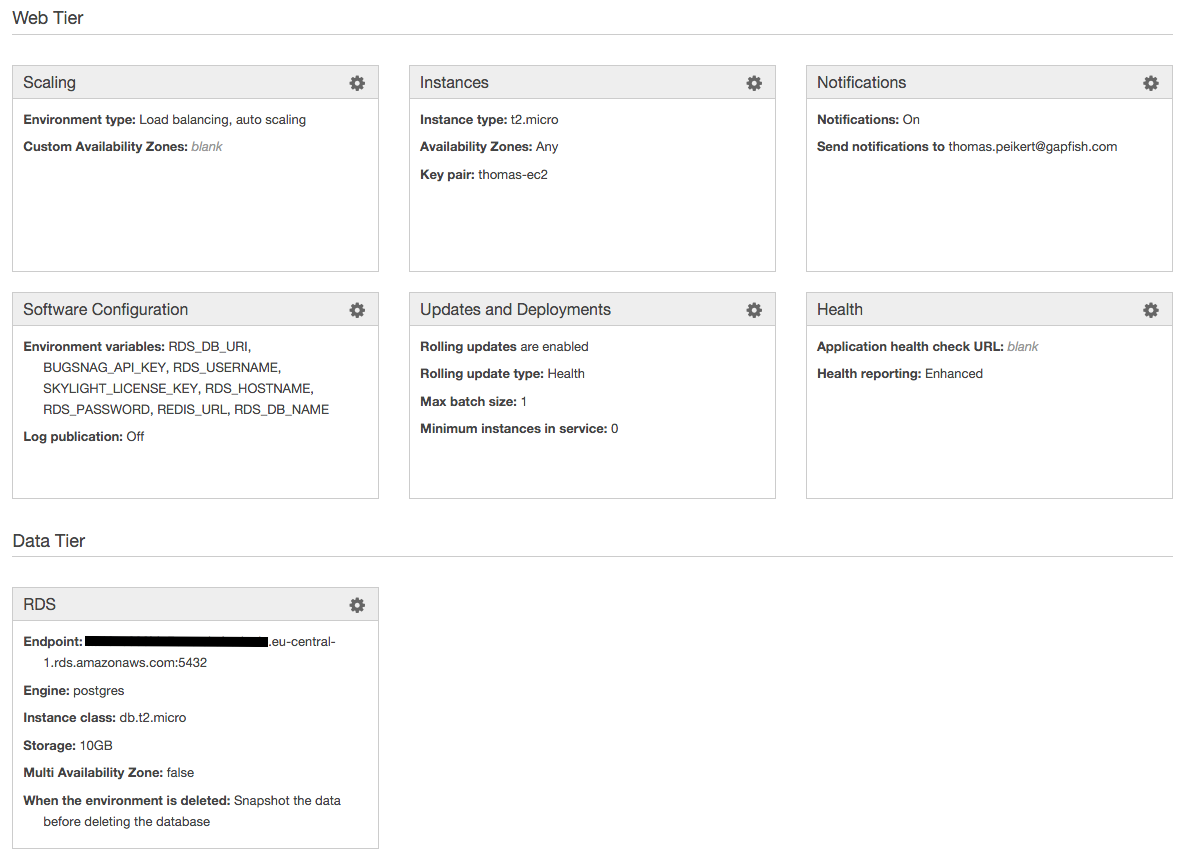
\includegraphics[width=\textwidth]{aws_config_ui}
\end{figure}
AWS EB ist selbst mit keinen Kosten verbunden, die Kosten ergeben sich ausschließlich aus den von EB genutzten Ressourcen, also die genutzten EC2 Instanzen und der reine Speicherverbrauch der Anwendung auf AWS S3. 

Elastic Beanstalk bildet hier einen Hybridansatz zwischen Iaas und Paas. Es wird lediglich eine komplette Anwendung mit Dependency Management hochgeladen und automatisiert deployt, nicht aber eine gesamte Maschine eingerichtet.
Die weiteren, von der Anwendung benötigten Ressourcen, werden jedoch, wie bei IaaS üblich, separat eingerichtet und verwaltet. Zum Einen ist dies eine PostgreSQL Datenbank und der Key-Value Store Redis. Hierfür bietet Amazon jeweils gesonderte Services zum Betrieb. Relationale Datenbanken können über den Amazon Relational Database Service (RDS)\cite{aws:rds} genutzt werden, Redis wird über Amazon ElastiCache\cite{aws:elasticache} angeboten. Beide Services bieten ebenso wie Elastic Beanstalk gute Skalierungsmöglichkeiten.

Bisher wurden die gesamte Firmenanwendung auf einem System, bei einem Hoster betrieben. Zwar gibt es durchaus separate Repositories, z.B. um eine API für die mobilen Anwendungen zu bieten, diese werden jedoch immer über das Ruby Webserver Interface Rack in die bestehende Anwendung eingebunden. So werden sie bei jedem Deploy der Hauptanwendung ebenfalls deployt. Weiterhin laufen sie im selben Prozess auf dem gleichen Server wie die Hauptanwendung. Hier ist also keinerlei separates Handling zum Monitoring notwendig. Es kann auch keinen Ausfall eines Teilsystems geben, da alle Teile zusammenhängen. Lediglich die Datenbanken und Redis laufen auf dedizierten Servern, diese werden aber im gleichen Netzwerk betrieben, somit sind zwar Teilausfälle möglich, diese werden durch ein Primary-Secondary System abgesichert, Netzwerkprobleme sind aber in der Regel ausgeschlossen. Das gesamte System kann wie in \autoref{fig:deployd} dargestellt werden.

\begin{figure}[!ht]
    \centering
    \caption{Deploymentdiagramm: Zusammenspiel aller Komponenten}
    \label{fig:deployd}
    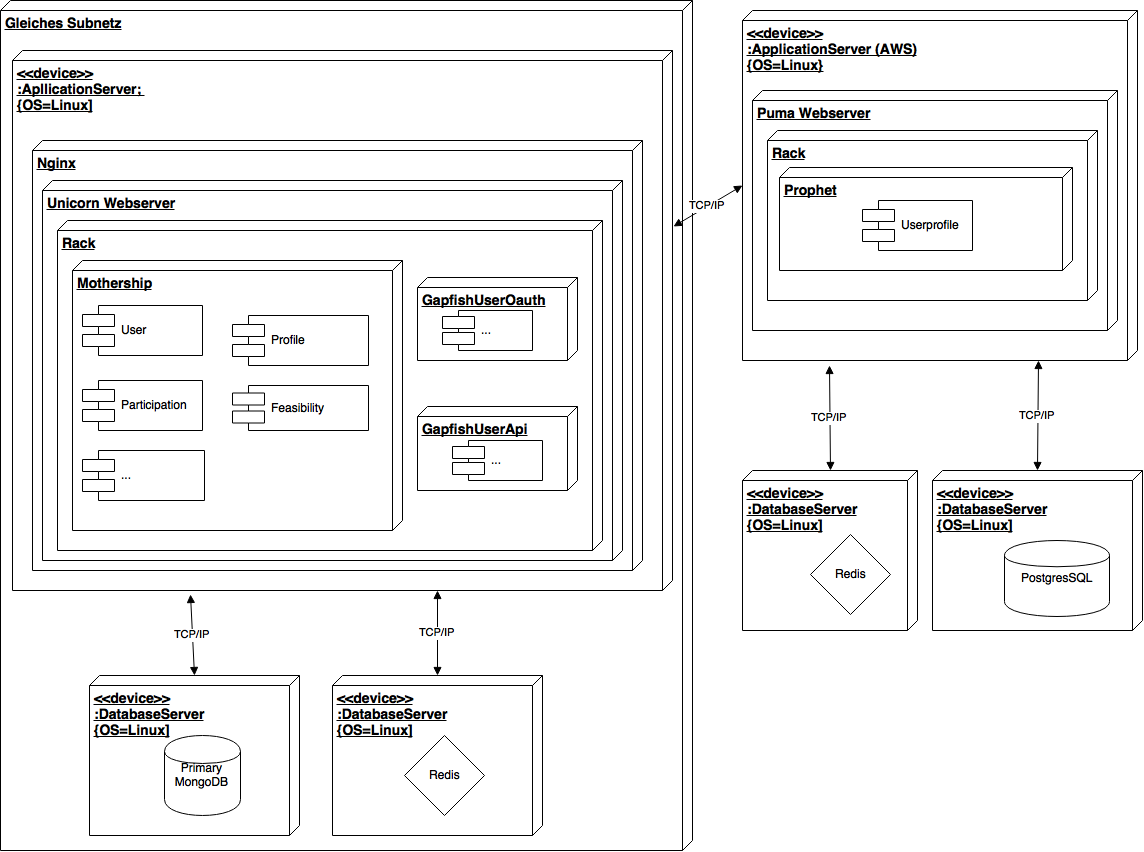
\includegraphics[width=\textwidth]{deploymentdiagram}
\end{figure}

Besonders wichtig für den Microservice ist daher das Monitoring der Anwendung und des Servers. Da hier ein von der Hauptanwendung komplett separates System betrieben wird, muss sichergestellt werden, dass zum Einen Fehler schnell erkannt und zum Anderen schnell behoben werden. 

Zum Monitoring nutze ich zum Einen Amazons eigene Monitoring Lösung, die über den Gesundheitsstatus der Anwendung informiert. Wechselt die Anwendung vom Gesundheitsstatus ``OK'' in einen anderen, werden die Entwickler direkt über eine Email informiert.

Zusätzlich zum allgemeinen Ausfallmonitoring durch Amazon, integrierte ich das Monitoring Tool Skylight\cite{skylight} in die Anwendung. Im bisherigen Betriebssetup wird aktuell NewRelic\cite{newrelic} zum Monitoring eingesetzt. Skylight zeichnet sich jedoch durch einen besonders geringen Overhead aus, was sich beim Microservice durchaus anbietet. Skylight informiert ebenfalls per Email über Ausfälle und zeichnet im Allgemeinen die Performance des Systems auf. So kann zu jedem Zeitpunkt der Vergangenheit, über Wochen hinweg, detailliert die Performance des Sytsems nachvollzogen werden. Zusätzlich zu allgemeinen Aufzeichnungen der Response Time, kann hier nach Datenbankabfragen unterschieden werden. So wird schnell deutlich, welche Anfragen besonders zeitintensiv sind und wo Handlungsbedarf oder Verbesserungsmöglichkeiten bestehen. 

Als Fehlerreporting Tool kommt im Microservice Bugsnag\cite{bugsnag} zum Einsatz. Bugsnag wird bereits als primäres Firmentool verwendet und eignet sich ebenfalls gut für kleine Anwendungen. Bugsnag zeichnet Fehler im System mit Stacktrace auf und informiert die Entwickler ebenfalls per Email.

Das Informieren über Fehler per Email ist im Unternehmen ein durchaus üblicher Weg, daher eignet sich diese Integration auch für den neuen Service. Weiterhin besteht in der Firma ein Dashboard, was zwar nicht die Performance des neuen Microservices an sich, aber die Gesamtperformance des Sampling Prozesses darstellt. Dieser umschließt alles vom Erstellen der Query, der Abfrage des neuen Services, bis hin zum Verarbeiten und Anzeigen der Queryergebnisse. So können Probleme auf dem Dashboard leicht von den Entwicklern bemerkt werden. All dies sind im Live Betrieb erprobte Techniken und eignen sich dadurch sehr gut für die Ausweitung auf neue Services.

\section{Analyse der Performance des Microservices}
Da der neue Microservice zum Zweck der Beschleunigung von Nutzerprofilqueries entwickelt wurde, ist hier insbesondere eine Auswertung der Geschwindigkeit des neuen Services angebracht. 
Zur Bewertung der Performance des neu entwickelten Microservies wurde die neue Datenbank mit Dummydaten gefüllt. Da im Rahmen der Bachelorarbeit aus Zeigründen kein vollständiges Ausformulieren des Schemas möglich war, wurden hier zusätzlich zu einigen wenigen echten Feldern, 165 Dummyspalten des Typs String angelegt. Anschließend wurden die Spalten mit 200.000 Nutzerdaten gefüllt. Dieser Datenbestand diente als Grundlage aller folgenden Performanceanalysen. Zum Vergleich dazu wurde in der Primärdatenbank Anfragen auf ein Panel beschränkt. Nutzer sind hier je nach Umfrageplatform, auf der sie sich registriert haben, in verschiedene Panels unterteilt. Das ``EC'' Panel umfasst hier ebenfalls rund 200.000 registrierte Nutzer und diente als Grundlage der Vergleiche.
Beim Vergleich der Performance muss hier grundlegend in zwei Arten der Queries unterschieden werden. Zum Einen sind dies Queries auf solche Spalten, die durch Indizes abgedeckt sind, zum Anderen auf solche Spalten, die nicht durch Indizes abgedeckt sind.

Hier muss explizit darauf hingewiesen werden das es sich bei den durchgeführten Tests um reine Performance Tests, nicht aber Load oder Stress Tests handelt.
Um die Testergebnisse möglichst repräsentativ zu halten, wurde hier im Live System getestet.\cite{msdn:perftesting} 
Da eine vollkommene Lastfreiheit des bestehenden Live Systems schlicht unmöglich ist, wurden hier Testzeitpunkte mit möglichst geringer Last gewählt. Vor Tests wurde immer explizit sichergestellt, dass aktuell keine Berechnungen o.Ä. laufen. Dies war in der Regel in den frühen Morgenstunden (vor 7 Uhr) am besten möglich.
Für den entwickelten Microservice war Lastfreiheit leicht zu garantieren, da der Zugriff, wie bereits beschrieben, über Feature Toggling kontrolliert wurde. 

Die Performance Tests wurden immer vom bestehenden Live System aus gestartet. Hierzu wurde eine SSH Verbindung aufgebaut und anschließend eine Ruby Konsole gestartet. Hier wurden direkt die QueryExecuter Subklassen des MongoidQueriers und des ProphetQueriers genutzt. Dies ist eine angebrachte Stelle zum Testen, da genau an dieser Stelle zwischen den beiden Features getoggled wird. Der restliche Ablauf ist im System identisch.

Um die Performance des Microservices messen zu können, wurde dieser leicht angepasst. Da das Fehlerhandling noch nicht ausreichend integriert ist, wurde der Microservice hier auf eine synchrone Berechnung umgestellt. Die Hauptanwendung erhält den Zugriffsschlüssel also erst, wenn die Abfrage auf die Datenbank abgeschlossen ist. Dadurch wird zwar ggf. etwas Zeit für über die synchronen Netzwerkaufrufe verloren, die Messung der echten Queryzeit ist dadurch aber erst verlässlich möglich.

Zum Messen der Performance wird hier die Ruby eigene Klasse ``Benchmark'' genutzt. Sie bietet sich für einfache Zeitmessungen an. 
Es wurden diverse, für die Anwendung typische, Queries gebildet und als Selector formuliert. Jede Query wurde anschließend an die jeweiligen Klassen des MongoidQueriers und des ProphetQueriers übergeben. Abschließend wurde die Population (COUNT) und die \textit{response rates} (SELECT) abgefragt. Queries wurden jeweils 100 mal ausgeführt. Die in \autoref{fig:perftesttable} aufgelisteten Zahlen beziehen sich auf den daraus errechneten Durchschnitt einer einzelnen Query.

\begin{figure}[!ht]
    \centering
    \caption{Performance Tests diverser Queries: MongoDB vs. SQL API}
    \label{fig:perftesttable}
    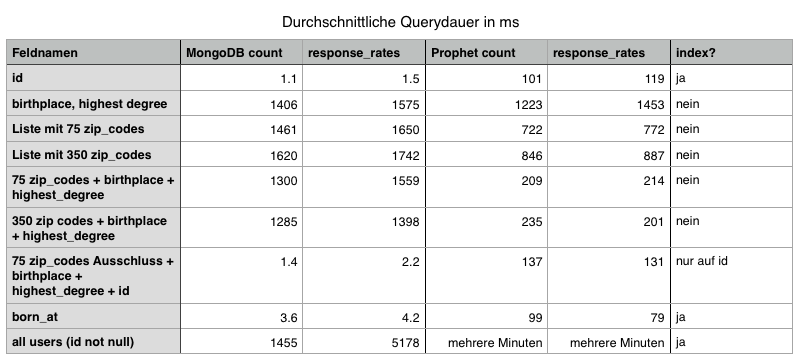
\includegraphics[width=\textwidth]{performance_table}
\end{figure}

Besonders auffällig sind die Zeitunterschiede zwischen den Abfragen der simplen Zahlen (COUNT) und dem Abfragen konkreter Daten (SELECT), wie \textit{ids} oder \textit{response rates}. Hier zeigen sich im Gegensatz zu MongoDB im Microservice keine signifikanten Zeitunterschiede. Dies ist auf die Abarbeitung der Query im Microservice zurückzuführen. Damit nur eine Query ausgeführt wird, werden hier alle erforderlichen Daten (\textit{ids}, \textit{response rates}, \textit{response rate sum} und \textit{count}) in einem Schritt aufbereitet. Es werden hierfür immer \textit{ids} und \textit{response rates} aus der Datenbank abgerufen. Anschließend werden diese gezählt und die die \textit{response rate sum} gebildet. Dadurch kommen Unterschiede lediglich durch Latenzvariation und ggf. Bilden der JSON Antwort zustande.
In jedem Fall sollte darüber nachgedacht werden, inwiefern hier Optimierungen möglich sind. Eventuell bietet es sich an, die einzelnen Schritte wie in MongoDB aufzusplitten. Hierdurch würden sich aber vier Queries ergeben. Mitunter wären hier die COUNTs dann früher bereit, im Lebenszyklus eines Projektes werden jedoch immer alle Daten benötigt, demnach macht dies nur bedingt Sinn. 

Auffällig ist hier auch das Abfragen aller ids (\textit{id not null}). Hier kommt es zu extremen Laufzeiten beim Microservice. Dies ist vermutlich eher ein Problem im Code, als bei der Datenbankabfrage an sich und daher behebbar. Es scheint auf die Hohe Zahl der Daten zurückzuführen zu sein (200.000). Bei den anderen Queries wurden in der Regel bis 20.000 Ergebnisse zurückgegeben. Dies geht über die üblichen Problemgrößen in der Anwendung bereits hinaus und ist daher für den Vergleich ausschlaggebend.

Nichtsdestotrotz hat man im Microservice auch relativ hohe Queryzeiten. Bei einer Requestlaufzeit von 50ms wird hier im ersten Schritt beim asynchronen Queryen der API immer ein Fehler auftreten. Demnach wären hier immer mehrere Requests notwendig. Ggf. bietet es sich an, hier einen initialen Timeout auf Basis der durchschnittlichen Berechnungslaufzeit einzurichten, um unnötige Requests zu sparen. Ein beibehalten des synchronen Abarbeitens und direktes zurückgeben der errechneten Daten würde gegen die REST Spezifikation verstoßen und wurde daher zunächst ausgeschlossen, wäre aber für die Zukunft durchaus denkbar.

\begin{figure}[!ht]
    \centering
    \caption{Durchschnittliche Query Laufzeiten in ms: index vs no index, count vs. select}
    \label{fig:perftestgraph}
    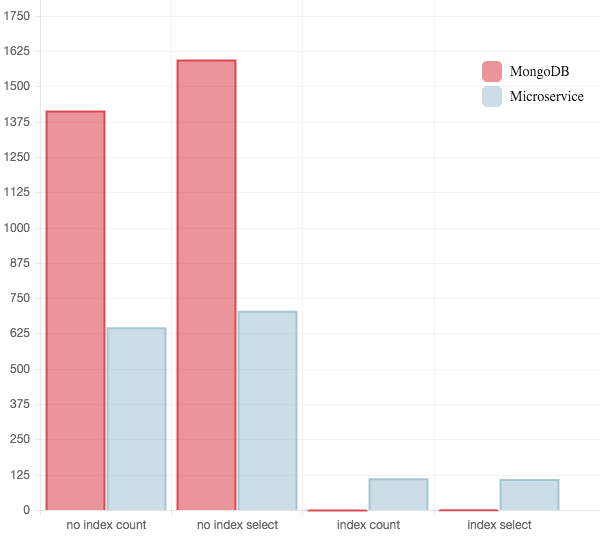
\includegraphics[width=\textwidth]{performance_graphs}
\end{figure}

Im Allgemeinen wird aber ein Trend sichtbar. Bei üblichen Queries mit normalen Resultatgrößen auf Felder ohne Indizes kann schon jetzt Zeit gewonnen werden. Dies wird nur besser, wenn hier in PostgreSQL Indizes angelegt werden. 
Auf Felder die in MongoDB bereits durch Indizes abgedeckt sind, kann hier keine Zeit gewonnen werden. Zwar sind diese Requests im neuen Service auch sehr schnell, aber der einfache Overhead durch die Netzwerkkommunikation lässt hier eine höhere Zeit zustande kommen.
Dies ist zwar nicht optimal, aber ein durchaus akzeptabler Tradeoff im Unternehmen. Wichtig ist hier eine konstant gute Performance. Die bereits erreichten Verbesserungen sind hier ein guter Anfang.
Weiterhin ist darauf hinzuweisen, dass es sich hier im bestehenden um einen fast lastfreien Zustand handelte. Unter Last im Betrieb, mit Locking der Datenbanken bei Änderungen an Userprofilen, Replication Lag und weitere Last auf der Datenbank durch andere Operationen kommen hier mitunter teilweise sehr lange Query Laufzeiten zustande. 
Der Microservice nutzt auf weiterhin AWS bisher die kleinsten Instanzgrößen, keinerlei Replikation oder Skalierung und keinerlei Indizes außer die zum Testen angelegten. 
Hier ist davon auszugehen, dass Optimierungen, wie sie auch in der Hauptanwendung genutzt werden, also Replikationen und größere Instanzen, noch Verbesserungen erzielen können. Gerade über Indizes, die in MongoDB bereits alle in Benutzung sind, ist hier von einer Verbesserung der Performance gegenüber der Hauptanwendung auszugehen. Weiterhin sollte sich der Microservice einwandfrei skalieren lassen. Hier kann durch einfache X-Achsen Skalierung (funktional identische Replikas), vor allem der Datenbanken, gutes Lastmanagament erzielen.
All dies, ebenso wie Varianzen in den Querylaufzeiten, Analyse des 95. Percentils, hinzfügen von Indizes auf PostgreSQL etc., wurden in dieser kurzen Performance Analyse nicht berücksichtigt. Sie soll nur ein generelles Gefühl für die gewonnene Performance des bei Weitem noch nicht fertigen Prototyps vermitteln.